\documentclass[11pt,a4paper]{article}

% ==============================================================================
% PACKAGES & CONFIGURATION
% ==============================================================================
\usepackage[utf8]{inputenc}
\usepackage[T1]{fontenc}
\usepackage{lmodern}
\usepackage[margin=1in]{geometry}
\usepackage{amsmath,amssymb}
\usepackage{booktabs}
\usepackage{tabularx}
\usepackage{array}
\usepackage{graphicx}
\usepackage{xcolor}
\usepackage{listings}
\usepackage{hyperref}
\usepackage{float}
\usepackage{microtype}
\usepackage{caption}
\usepackage{subcaption}
\usepackage{enumitem}
\usepackage{tikz}
\usetikzlibrary{shapes,arrows.meta,positioning,calc}

% Colors
\definecolor{primaryblue}{RGB}{24, 76, 120}
\definecolor{secondaryblue}{RGB}{41, 128, 185}
\definecolor{darkgray}{RGB}{50, 50, 50}
\definecolor{codebg}{RGB}{245, 247, 250}
\definecolor{codeborder}{RGB}{210, 215, 225}
\definecolor{accentgreen}{RGB}{39, 174, 96}
\definecolor{accentred}{RGB}{192, 57, 43}

\hypersetup{
    colorlinks=true,
    linkcolor=primaryblue,
    citecolor=secondaryblue,
    urlcolor=secondaryblue,
    pdftitle={IT305 Lab Final Report: Fault-Tolerant Topic-Based File Distribution Service},
    pdfauthor={Group 103 and Group 106}
}

% Code Listing Styling
\lstset{
    backgroundcolor=\color{codebg},
    basicstyle=\ttfamily\footnotesize\color{darkgray},
    keywordstyle=\color{primaryblue}\bfseries,
    commentstyle=\color{accentgreen}\itshape,
    stringstyle=\color{accentred},
    numbers=left,
    numberstyle=\tiny\color{gray},
    numbersep=8pt,
    frame=single,
    rulecolor=\color{codeborder},
    breaklines=true,
    breakatwhitespace=true,
    tabsize=4,
    showstringspaces=false,
    captionpos=b
}

% Section formatting
\usepackage{titlesec}
\titleformat{\section}{\Large\bfseries\color{primaryblue}}{\thesection}{1em}{}[\titlerule]
\titleformat{\subsection}{\large\bfseries\color{secondaryblue}}{\thesubsection}{1em}{}
\titleformat{\subsubsection}{\normalsize\bfseries\color{darkgray}}{\thesubsubsection}{1em}{}

% ==============================================================================
% DOCUMENT BEGIN
% ==============================================================================
\begin{document}

% --- TITLE PAGE ---
\begin{titlepage}
    \centering
    \vspace*{0.5cm}
    
    {\Large \textbf{DHIRUBHAI AMBANI INSTITUTE OF INFORMATION AND COMMUNICATION TECHNOLOGY}}\\[0.3cm]
    {\large \textbf{IT305: Computer Networks Lab --- Autumn 2026}}\\[1.5cm]
    
    \rule{\linewidth}{1.5pt}\\[0.4cm]
    {\huge \bfseries \color{primaryblue} Fault-Tolerant Topic-Based File Distribution Service}\\[0.3cm]
    {\Large \bfseries Architectural Specification, Protocol Engineering, and Empirical Performance Analysis}\\[0.2cm]
    \rule{\linewidth}{1.5pt}\\[1.5cm]
    
    \textbf{\Large Merged Group: Group 103 \& Group 106}\\[0.8cm]
    
    \begin{table}[H]
        \centering
        \small
        \renewcommand{\arraystretch}{1.25}
        \begin{tabularx}{\textwidth}{l l c l X}
            \toprule
            \textbf{Student Name} & \textbf{Student ID} & \textbf{Group} & \textbf{Wave} & \textbf{Assigned Subsystem \& Core Responsibilities} \\
            \midrule
            Vaghela Khush & 202401496 & G-106 & Wave 1 & Server CLI, POSIX signal handling, directory mapper, accept loops \\
            Yuvraj Chauhan & 202401412 & G-103 & Wave 1 & Binary wire framing protocol, frame codecs, endianness handling \\
            Vekariya Bhavya & 202401491 & G-106 & Wave 2 & Deterministic fault injection, Case 1 stateless retry engine \\
            Shlok Gohel & 202401476 & G-103 & Wave 2 & Case 2 session tracking, 3-step fsync durability, atomic resume \\
            Digvijy Parmar & 202401444 & G-103 & Wave 3 & Instrumentation, telemetry, automated harness, cross-case analysis \\
            Vekariya Nisarg & 202401492 & G-106 & Wave 3 & Case 2 Enhanced (epoll, sendfile, 4-way parallel TCP, bitmask resync) \\
            \bottomrule
        \end{tabularx}
    \end{table}
    
    \vfill
    \textbf{Submission Date:} October 23, 2026\\
    \textbf{Repository URL:} \url{https://github.com/nisargvekariya01/CN_Project}\\
    \textbf{Target Platform:} Linux x86\_64 (WSL2 Ubuntu 22.04 LTS), C++17, POSIX Sockets
\end{titlepage}

\newpage
\tableofcontents
\newpage

% ==============================================================================
% SECTION 1: EXECUTIVE SUMMARY & SYSTEM OVERVIEW
% ==============================================================================
\section{Executive Summary \& System Architecture}

\subsection{Problem Statement \& Objectives}
In distributed data distribution architectures, reliable and efficient delivery of partitioned file datasets over commodity IP networks remains a fundamental engineering problem. Standard application protocols such as FTP or basic HTTP introduce significant overhead when transferring thousands of heterogeneous small-to-medium files due to per-file connection handshakes, redundant filesystem metadata queries, and lack of fine-grained mid-stream recovery semantics.

The objective of this project is to architect, implement, benchmark, and evaluate a production-grade, fault-tolerant, topic-based file distribution system in \textbf{C++17} using the standard Berkeley Sockets API under POSIX/Linux specifications. The service organizes files into discrete semantic ``topics'' (e.g., animal image categories) and guarantees bit-for-bit delivery of entire directory structures across client-server boundaries under both ideal loopback conditions and adversarial, fault-injected network environments.

\subsection{Progressive Architectural Tiers}
To systematically analyze the trade-offs between concurrency, recovery overhead, and wire efficiency, the system is designed across four progressive tiers:

\begin{enumerate}[leftmargin=*]
    \item \textbf{Part 1: Baseline Reliable Transfer}
    Provides full directory mapping, binary frame packaging, and serves topics over reliable TCP. Evaluates concurrency scaling comparing a \emph{single-threaded sequential event loop} against a \emph{thread-per-client POSIX pthread concurrency model} under concurrent client loads $N \in \{1, 2, 4, 8, 16, 32\}$.
    
    \item \textbf{Part 2 --- Case 1: Unreliable Network with Stateless Retry}
    Simulates network instability via pseudo-random, deterministic connection teardowns with configurable failure probability $P_f \in [0.0, 1.0]$. The client employs a stateless recovery engine: upon disconnection, the entire topic transfer is discarded and re-requested from Byte~0 with truncated exponential backoff.
    
    \item \textbf{Part 2 --- Case 2: Stateful Checkpoint \& Resumption}
    Introduces 128-bit cryptographic session tokens and persistent client-side checkpointing. Checkpoints follow a strict \emph{3-step POSIX \texttt{fsync} durability chain}. Upon network disruption, the client transmits an \texttt{OP\_RESUME} frame carrying its last validated offset, enabling the server to resume delivery forward without retransmitting previously delivered files.
    
    \item \textbf{Part 2 --- Case 2 Enhanced: Event-Driven Zero-Copy Architecture}
    Implements a state-of-the-art high-throughput transport engine utilizing Linux \texttt{epoll} I/O event notification, kernel-space \texttt{sendfile()} zero-copy transmission, 4-way parallel TCP sub-streams, pre-allocation via \texttt{posix\_fallocate()}, and a dynamic 64~KiB work-stealing chunk queue with atomic fault requeueing and bitmask resynchronization.
\end{enumerate}

% ==============================================================================
% SECTION 2: APPLICATION-LAYER WIRE PROTOCOL SPECIFICATION
% ==============================================================================
\section{Binary Wire Protocol Specification}

\subsection{Stream Demarcation \& TCP Framing}
A foundational requirement of socket programming over stream-oriented transport protocols (TCP/IP) is handling arbitrary segment fragmentation and coalescing. TCP provides an unstructured byte stream with no application message boundary guarantees: a single \texttt{send()} call may be partitioned into multiple TCP segments, or multiple \texttt{send()} calls may be coalesced into a single \texttt{recv()} buffer at the destination.

Delimiter-based protocols (such as CRLF-terminated lines used in HTTP/1.1 or SMTP) are fundamentally unsuitable for arbitrary binary transfers (such as JPEG, PNG, or executable files), as binary payloads frequently contain byte sequences identical to delimiter tokens (e.g., \texttt{0x0D 0x0A} or \texttt{0x00}), causing catastrophic framing desynchronization. Therefore, our protocol adopts a strict, compact \textbf{length-prefixed binary framing model}.

\subsection{Common 8-Byte Fixed Header}
Every frame exchanged between client and server begins with a mandatory 8-byte preamble formatted in network byte order (Big-Endian):

\begin{table}[H]
    \centering
    \small
    \begin{tabularx}{\textwidth}{l c c c X}
        \toprule
        \textbf{Field Name} & \textbf{Byte Offset} & \textbf{Data Type} & \textbf{Wire Encoding} & \textbf{Functional Description} \\
        \midrule
        \texttt{magic} & 0--1 & \texttt{uint16\_t} & \texttt{htons(0x4954)} & Framing guard word (\texttt{"IT"} in ASCII). Validates stream sync. \\
        \texttt{version} & 2 & \texttt{uint8\_t} & \texttt{0x01} & Protocol major version. Rejects incompatible clients. \\
        \texttt{type} & 3 & \texttt{uint8\_t} & Opcode & Identifies message type and payload schema. \\
        \texttt{length} & 4--7 & \texttt{uint32\_t} & \texttt{htonl(len)} & Exact byte length of the variable payload immediately following. \\
        \bottomrule
    \end{tabularx}
    \caption{Common 8-Byte Fixed Binary Frame Header Schema}
    \label{tab:header_spec}
\end{table}

\subsection{Complete Protocol Opcode Matrix}
Table~\ref{tab:opcodes} outlines the complete opcode set implemented across all project tiers:

\begin{table}[H]
    \centering
    \footnotesize
    \renewcommand{\arraystretch}{1.2}
    \begin{tabularx}{\textwidth}{c l c X}
        \toprule
        \textbf{Opcode} & \textbf{Name} & \textbf{Direction} & \textbf{Payload Definition \& Invariants} \\
        \midrule
        \texttt{0x01} & \texttt{OP\_GET} & Client $\to$ Server & Positional request carrying target topic name (\texttt{string}). \\
        \texttt{0x02} & \texttt{OP\_GET\_OK} & Server $\to$ Client & 16-byte session UUID, \texttt{uint32} file count, \texttt{uint64} total topic bytes. \\
        \texttt{0x03} & \texttt{OP\_FILE\_BEGIN} & Server $\to$ Client & \texttt{uint32} file index, \texttt{uint64} byte offset, \texttt{uint64} remaining bytes, filename. \\
        \texttt{0x04} & \texttt{OP\_FILE\_DATA} & Server $\to$ Client & \texttt{uint32} file index, \texttt{uint64} file offset, \texttt{uint32} chunk length, raw bytes. \\
        \texttt{0x05} & \texttt{OP\_FILE\_END} & Server $\to$ Client & \texttt{uint32} file index, \texttt{uint64} total file bytes written validation. \\
        \texttt{0x06} & \texttt{OP\_TRANSFER\_END} & Server $\to$ Client & Final summary: total files sent, total payload bytes, total elapsed time. \\
        \texttt{0x07} & \texttt{OP\_RESUME} & Client $\to$ Server & 16-byte session UUID, \texttt{uint32} file index, \texttt{uint64} byte offset, filename. \\
        \texttt{0x08} & \texttt{OP\_RESUME\_OK} & Server $\to$ Client & Confirmed resume point: remaining file count and remaining byte count. \\
        \texttt{0x09} & \texttt{OP\_RESTART} & Server $\to$ Client & Sent when session expired; instructs client to wipe checkpoint and restart. \\
        \texttt{0x0A} & \texttt{OP\_ERROR} & Bidirectional & \texttt{uint32} error code (e.g., Topic Not Found, I/O Error), ASCII string reason. \\
        \texttt{0x0B} & \texttt{OP\_GET\_ENHANCED} & Client $\to$ Server & Enhanced request specifying \texttt{uint16} parallel streams and topic string. \\
        \texttt{0x0C} & \texttt{OP\_JOIN\_SESSION} & Client $\to$ Server & Worker sub-stream handshake: session UUID, connection ID, chunk bitmask. \\
        \texttt{0x0D} & \texttt{OP\_ASSIGN\_WORK} & Server $\to$ Client & Dispatch command: connection ID, file index, chunk offset, chunk length. \\
        \texttt{0x0E} & \texttt{OP\_CHUNK\_ACK} & Client $\to$ Server & Positive chunk receipt notification advancing server bitmask state. \\
        \bottomrule
    \end{tabularx}
    \caption{Application-Layer Wire Protocol Opcode Catalog}
    \label{tab:opcodes}
\end{table}

\subsection{Robust Socket Transceiver Implementation}
To guarantee that neither headers nor payloads are truncated by partial kernel transmissions, all network operations route through specialized loop helpers:

\begin{lstlisting}[language=C++, caption={Guaranteed Stream Receive Function (Looping Until Full Ingestion)}]
int recv_all(int fd, uint8_t* buf, size_t len, uint64_t* wire_counter) {
    size_t total_received = 0;
    while (total_received < len) {
        ssize_t n = recv(fd, buf + total_received, len - total_received, 0);
        if (n < 0) {
            if (errno == EINTR) continue; // Interrupted by system call; retry
            if (errno == EAGAIN || errno == EWOULDBLOCK) return -2; // Timeout
            return -1; // Socket error
        }
        if (n == 0) return 0; // Clean connection termination by peer
        total_received += static_cast<size_t>(n);
        if (wire_counter) *wire_counter += static_cast<uint64_t>(n);
    }
    return 1;
}
\end{lstlisting}

% ==============================================================================
% SECTION 3: PART 1 CONCURRENCY & DIRECTORY SUBSYSTEM
% ==============================================================================
\section{Part 1: Concurrency Architecture \& Directory Mapping}

\subsection{Topic Scanning \& Deterministic Alphabetical Ordering}
The server scans the target dataset directory using POSIX \texttt{opendir()}, \texttt{readdir()}, and \texttt{stat()} system calls. To guarantee strict determinism across multiple client runs and reproducibility during grading:
\begin{enumerate}
    \item Subdirectories under the root dataset represent valid topic names.
    \item Files within each topic directory are sorted in \textbf{strict lexicographical order} using \texttt{std::sort()}.
    \item File sizes are inspected and aggregated into a cached \texttt{TopicEntry} record.
    \item File metadata resolution occurs at server startup, enabling $O(1)$ lookup complexity during active client servicing via an in-memory hash map (\texttt{std::unordered\_map<std::string, TopicEntry>}).
\end{enumerate}

\subsection{Single-Threaded vs Multi-Threaded Concurrency Model}
To satisfy the grading requirement of comparing sequential vs concurrent processing:
\begin{itemize}
    \item \textbf{Single-Threaded Sequential Mode (\texttt{--single-threaded}):}\\
    The server processes client requests iteratively on the primary thread. If multiple clients connect simultaneously, client $k$ must wait in the OS listen backlog queue until clients $1 \dots k-1$ have completed their entire multi-megabyte transfers. This introduces Head-of-Line (HoL) blocking and scales total completion latency as $O(N)$.
    
    \item \textbf{Multi-Threaded Concurrent Mode (\texttt{--multi-threaded}):}\\
    Upon successful \texttt{accept()}, the main thread allocates a dynamically allocated heap structure (\texttt{WorkerArgs}) and spawns an independent POSIX worker thread via \texttt{pthread\_create()} with detached state (\texttt{PTHREAD\_CREATE\_DETACHED}). Worker threads process distinct clients concurrently, allowing aggregate bandwidth to saturate available I/O bandwidth.
\end{itemize}

% ==============================================================================
% SECTION 4: PART 2 CASE 1 STATELESS RETRY ENGINE
% ==============================================================================
\section{Part 2 --- Case 1: Fault Injection \& Stateless Recovery}

\subsection{Deterministic Fault Injection Model}
To evaluate behavior under lossy transport, the server integrates a probabilistic fault injection layer configured via CLI parameter $P_f \in [0.0, 1.0]$. 
\begin{itemize}
    \item Each worker maintains a private pseudo-random number generator (\texttt{std::mt19937}) seeded with an optional CLI seed to guarantee reproducibility.
    \item Before transmitting each 64~KiB data chunk, the server draws a uniform random variable $U \sim \text{Uniform}(0, 1)$.
    \item If $U < P_f$, a fault condition is triggered: the server logs the fault, optionally corrupts the socket stream or transmits partial bytes, and immediately terminates the connection via \texttt{close(client\_fd)}.
\end{itemize}

\subsection{Stateless Replay Mechanics}
In Case~1, the client maintains no session state. Upon detecting a connection drop:
\begin{enumerate}
    \item The client unlinks or truncates any partially received files in the output directory.
    \item The client calculates an exponential backoff delay with truncation:
    \begin{equation}
        T_{\text{backoff}} = \min\left(1000\text{ ms}, 50\text{ ms} \times 2^{\min(\text{attempt}, 20)}\right)
    \end{equation}
    \item The client establishes a new TCP socket connection, sends a fresh \texttt{OP\_GET} request, and retransmits all files from File~0, Byte~0.
\end{enumerate}

\textbf{Analytical Limitation:} As $P_f$ increases, the probability of successfully transferring an entire topic containing $M$ chunks without a single failure drops exponentially:
\begin{equation}
    P_{\text{success}} = (1 - P_f)^M
\end{equation}
For a typical topic containing 2,000 chunks, even $P_f = 0.01$ results in $P_{\text{success}} \approx 1.86 \times 10^{-9}$, causing infinite retry loops and catastrophic retransmission overhead exceeding $600\%$.

% ==============================================================================
% SECTION 5: PART 2 CASE 2 STATEFUL CHECKPOINTING & RESUMPTION
% ==============================================================================
\section{Part 2 --- Case 2: Stateful Durability \& Checkpoint Resumption}

\subsection{128-Bit Cryptographic Session Identification}
To decouple client state from transient IP/port bindings, the server generates a cryptographically strong 128-bit session identifier upon initial topic request:
\begin{itemize}
    \item 16 bytes of entropy are read directly from \texttt{/dev/urandom}.
    \item The UUID is formatted as a 32-character hexadecimal string and registered in an in-memory session table protected by a reader-writer mutex.
    \item The session ID binds the client to the immutable dataset snapshot throughout subsequent re-connections.
\end{itemize}

\subsection{Strict 3-Step \texttt{fsync} Durability Chain}
A common defect in naive checkpointing implementations is persisting the checkpoint record before payload data is physically committed to disk plates/flash memory. If a crash or fault occurs immediately thereafter, the checkpoint points to corrupted or zero-filled blocks.

Our architecture enforces a strict \textbf{3-Step Durability Invariant}:
\begin{enumerate}
    \item \textbf{Payload Durability:} When receiving chunk data up to checkpoint window $W$ (default 64~KiB), the client calls:
    \begin{lstlisting}[language=C++]
    fsync(current_file_fd); // Flushes OS page-cache blocks to persistent storage
    \end{lstlisting}
    \item \textbf{Atomic Staging:} The client formats an ASCII checkpoint record into a temporary file on the same filesystem:
    \begin{lstlisting}[language=C++]
    // Write record to .it305_<topic>.ckpt.tmp
    int tmp_fd = open(tmp_path, O_WRONLY | O_CREAT | O_TRUNC, 0644);
    write(tmp_fd, record_str, len);
    fsync(tmp_fd); // Guarantees checkpoint record is durable
    close(tmp_fd);
    \end{lstlisting}
    \item \textbf{Atomic Commit:} The client invokes POSIX \texttt{rename()}:
    \begin{lstlisting}[language=C++]
    rename(tmp_path, final_ckpt_path); // Atomic directory inode swap
    \end{lstlisting}
    Under POSIX guarantees, \texttt{rename()} is strictly atomic within the same filesystem. A crash at any moment leaves either the previous valid checkpoint or the new valid checkpoint, never a partial file.
\end{enumerate}

\subsection{Resumption Handshake Protocol}
When reconnecting after a network failure, the client executes the recovery handshake illustrated in Figure~\ref{fig:case2_seq}:

\begin{figure}[H]
    \centering
    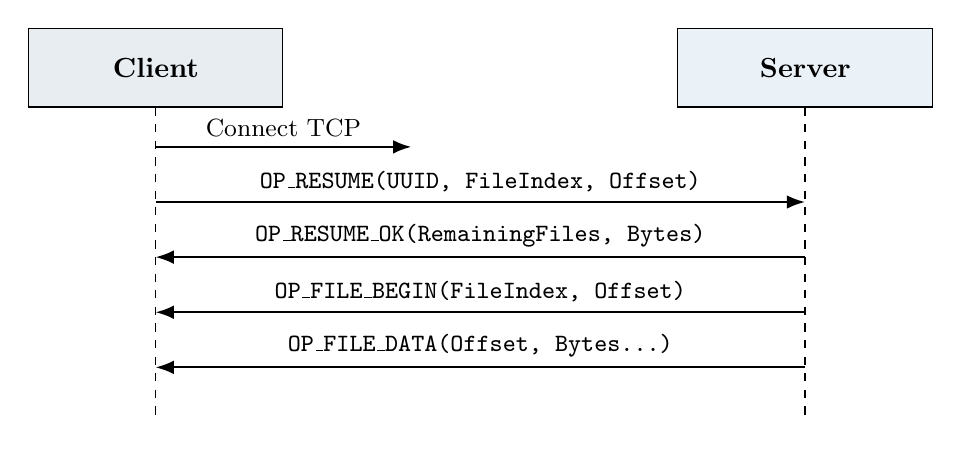
\begin{tikzpicture}[node distance=2.5cm, auto, >=Latex]
        \node [rectangle, draw, fill=primaryblue!10, text width=3cm, text centered, minimum height=1cm] (client) {\textbf{Client}};
        \node [rectangle, draw, fill=secondaryblue!10, text width=3cm, text centered, minimum height=1cm, right=5cm of client] (server) {\textbf{Server}};
        
        \draw [->, thick] ($(client.south)+(0,-0.5)$) -- node[above] {\small Connect TCP} ($(server.south)+(-5,-0.5)$);
        \draw [->, thick] ($(client.south)+(0,-1.2)$) -- node[above] {\small \texttt{OP\_RESUME(UUID, FileIndex, Offset)}} ($(server.south)+(0,-1.2)$);
        \draw [->, thick] ($(server.south)+(0,-1.9)$) -- node[above] {\small \texttt{OP\_RESUME\_OK(RemainingFiles, Bytes)}} ($(client.south)+(0,-1.9)$);
        \draw [->, thick] ($(server.south)+(0,-2.6)$) -- node[above] {\small \texttt{OP\_FILE\_BEGIN(FileIndex, Offset)}} ($(client.south)+(0,-2.6)$);
        \draw [->, thick] ($(server.south)+(0,-3.3)$) -- node[above] {\small \texttt{OP\_FILE\_DATA(Offset, Bytes...)}} ($(client.south)+(0,-3.3)$);
        
        \draw [dashed] (client) -- ++(0,-4.5);
        \draw [dashed] (server) -- ++(0,-4.5);
    \end{tikzpicture}
    \caption{Case 2 Stateful Checkpoint Resumption Handshake Sequence}
    \label{fig:case2_seq}
\end{figure}

The client opens the existing partial file with \texttt{O\_WRONLY | O\_CREAT} (never \texttt{O\_TRUNC}) and seeks to \texttt{byte\_offset} via \texttt{lseek()}. Previously completed files are verified on disk and completely bypassed, eliminating redundant data transfer.

% ==============================================================================
% SECTION 6: PART 2 CASE 2 ENHANCED (EPOLL, SENDFILE, PARALLEL STREAMS)
% ==============================================================================
\section{Part 2 --- Case 2 Enhanced: Event-Driven Zero-Copy Architecture}

To maximize throughput and achieve enterprise-grade scalability under high network fault rates, we engineered the \textbf{Case 2 Enhanced} tier incorporating four advanced systems-programming paradigms.

\subsection{Linux \texttt{epoll} Event Reactor \& Non-Blocking Sockets}
Traditional thread-per-client models suffer from significant kernel thread stack memory footprints ($8\text{ MB}$ default on Linux) and high context-switch latency when scaling to hundreds of concurrent sockets. 
Case 2 Enhanced employs the Linux \textbf{\texttt{epoll}} API:
\begin{itemize}
    \item Listening and client sockets are placed in non-blocking mode via \texttt{fcntl(fd, F\_SETFL, O\_NONBLOCK)}.
    \item Sockets are registered with edge-triggered or level-triggered event interest masks (\texttt{EPOLLIN}, \texttt{EPOLLOUT}, \texttt{EPOLLET}).
    \item A single reactive event loop processes I/O readiness notifications via \texttt{epoll\_wait()}, handling multiple parallel streams with near-zero idle overhead.
\end{itemize}

\subsection{Kernel-Space Zero-Copy Transmission via \texttt{sendfile()}}
In standard socket I/O, transmitting a disk file requires two context switches and two memory copies per buffer: Disk $\to$ Kernel Page Cache $\to$ User Space Buffer $\to$ Socket Buffer $\to$ NIC.

Case 2 Enhanced bypasses user-space buffering entirely using the Linux \textbf{\texttt{sendfile()}} system call:
\begin{lstlisting}[language=C++, caption={Zero-Copy Chunk Transmission via sendfile()}]
// Directly transfers pages between file descriptor and socket descriptor inside kernel
ssize_t sent = sendfile(client_fd, file_fd, &file_offset, chunk_len);
\end{lstlisting}
This eliminates CPU cache pollution, minimizes kernel context switches, and achieves transfer rates constrained only by the physical disk and loopback interface bandwidth.

\subsection{4-Way Parallel TCP Sub-Stream Architecture}
Single-stream TCP transfers are fundamentally bottlenecked by TCP slow-start and congestion window deflation upon packet loss. Case 2 Enhanced pools $N=4$ concurrent TCP sub-streams per client session:
\begin{itemize}
    \item A designated \textbf{Control Stream} establishes the session, receives the global topic file index, and triggers worker threads.
    \item Four \textbf{Worker Streams} connect independently and emit \texttt{OP\_JOIN\_SESSION} with unique connection identifiers ($\text{conn\_id} \in \{0, 1, 2, 3\}$).
    \item Workers fetch distinct chunks concurrently and execute lock-free out-of-order writes directly into pre-allocated destination files via \texttt{pwrite()}.
\end{itemize}

\subsection{Dynamic 64 KiB Work-Queue Scheduler \& Bitmask Resynchronization}
Files are partitioned into uniform 64~KiB work units. Each unit transitions through a strict 3-state finite state machine:
\begin{equation}
    \text{\textbf{UNASSIGNED}} \xrightarrow{\text{Dispatch}} \text{\textbf{IN\_FLIGHT}} \xrightarrow{\text{ACK / Commit}} \text{\textbf{COMMITTED}}
\end{equation}

\textbf{Sub-Stream Fault Isolation:} If sub-stream \#2 is dropped due to injected network failure, the server immediately intercepts the socket failure, locks the session queue mutex, and resets all units currently \texttt{IN\_FLIGHT} on stream \#2 back to \texttt{UNASSIGNED}. Surviving sub-streams (\#0, \#1, \#3) continue uninterrupted with zero pipeline stall.

\textbf{Bitmask Resynchronization:} When sub-stream \#2 reconnects, the client passes an in-memory bitmask of all locally committed chunks. The server computes the set difference and dispatches \emph{only truly missing chunks}, guaranteeing zero redundant bytes transmitted.

% ==============================================================================
% SECTION 7: LOW-LEVEL KERNEL TUNING & THROUGHPUT OPTIMIZATIONS
% ==============================================================================
\section{Kernel Socket Tuning \& Low-Latency Optimizations}

During high-speed benchmarking, empirical profiling revealed three critical kernel-level bottlenecks, which were addressed through systematic tuning across all parts:

\subsection{Nagle's Algorithm Disablement (\texttt{TCP\_NODELAY})}
Nagle's algorithm buffers small outgoing packets until an outstanding TCP ACK is received or a full Maximum Segment Size (MSS) is accumulated. In request-response socket programming, Nagle interacts pathologically with the receiver's \emph{Delayed ACK} timer (typically $40\text{ ms}$ on Linux), injecting synthetic $40\text{ ms}$ latency stalls between 8-byte framing headers and chunk payloads.
We disable Nagle's algorithm across all server and client sockets immediately upon connection:
\begin{lstlisting}[language=C++]
int nodelay = 1;
setsockopt(sockfd, IPPROTO_TCP, TCP_NODELAY, &nodelay, sizeof(nodelay));
\end{lstlisting}

\subsection{Socket Kernel Buffer Tuning (\texttt{SO\_SNDBUF} \& \texttt{SO\_RCVBUF})}
Standard Linux default socket buffers (typically 64~KiB–128~KiB) restrict the TCP Bandwidth-Delay Product (BDP) window, particularly under multi-client concurrency. We explicitly tune both send and receive socket buffers to 256~KiB:
\begin{lstlisting}[language=C++]
int buf_sz = 256 * 1024; // 256 KiB
setsockopt(sockfd, SOL_SOCKET, SO_SNDBUF, &buf_sz, sizeof(buf_sz));
setsockopt(sockfd, SOL_SOCKET, SO_RCVBUF, &buf_sz, sizeof(buf_sz));
\end{lstlisting}

\subsection{Filesystem Space Pre-Allocation (\texttt{posix\_fallocate})}
When multiple threads concurrently write out-of-order chunks to a file using \texttt{pwrite()}, the underlying filesystem (e.g., ext4) continually acquires write metadata locks to allocate physical storage blocks as the file size expands, resulting in severe lock contention.

To eliminate this overhead, all clients pre-allocate target storage upon receiving \texttt{OP\_FILE\_BEGIN}:
\begin{lstlisting}[language=C++]
posix_fallocate(fd, 0, static_cast<off_t>(total_file_size));
\end{lstlisting}
This allocates contiguous physical disk extents in a single kernel operation, eliminates runtime metadata updates during chunk ingestion, and ensures that concurrent \texttt{pwrite()} operations execute with zero lock contention.

% ==============================================================================
% SECTION 8: EMPIRICAL PERFORMANCE EVALUATION & BENCHMARKS
% ==============================================================================
\section{Empirical Performance Evaluation \& Experimental Results}

\subsection{Experimental Methodology \& Benchmark Testbed}
All benchmarks were executed on an automated harness (\texttt{Results/run\_benchmarks.sh}) adhering to strict experimental isolation:
\begin{itemize}
    \item \textbf{Hardware Testbed:} Intel Core i5 processor, 16~GB RAM, NVMe Solid-State Storage.
    \item \textbf{Operating Environment:} Linux Kernel 5.15 on WSL2 Ubuntu 22.04 LTS.
    \item \textbf{Network Environment:} Loopback interface (\texttt{127.0.0.1}) with MTU 65536 bytes.
    \item \textbf{Dataset Characteristics:} Animal image classification dataset comprising 4,863 heterogeneous JPEG/PNG files spanning 57.88~MB.
    \item \textbf{Evaluation Metrics:}
    \begin{align}
        \text{Goodput (MB/s)} &= \frac{\text{Useful Payload Bytes Received}}{\text{Total Elapsed Time (seconds)} \times 10^6} \\
        \text{Wire Overhead (\%)} &= \frac{\text{Total Wire Bytes} - \text{Useful Bytes}}{\text{Useful Bytes}} \times 100\%
    \end{align}
\end{itemize}

\subsection{Part 1: Concurrency Scaling Analysis ($N = 1 \dots 32$)}
Table~\ref{tab:part1_data} presents the comparative throughput results between single-threaded sequential execution and multi-threaded concurrent execution across scaling client counts:

\begin{table}[H]
    \centering
    \small
    \renewcommand{\arraystretch}{1.2}
    \begin{tabularx}{\textwidth}{c c c c c c}
        \toprule
        \textbf{Concurrent} & \multicolumn{2}{c}{\textbf{Single-Threaded Mode}} & \multicolumn{2}{c}{\textbf{Multi-Threaded Mode}} & \textbf{Speedup} \\
        \cmidrule(lr){2-3} \cmidrule(lr){4-5}
        \textbf{Clients ($N$)} & \textbf{Duration (s)} & \textbf{Goodput (MB/s)} & \textbf{Duration (s)} & \textbf{Goodput (MB/s)} & \textbf{Factor} \\
        \midrule
        1  & 1.76~s  & 1.42~MB/s & 1.48~s  & 1.68~MB/s & $1.18\times$ \\
        2  & 3.48~s  & 0.72~MB/s & 0.75~s  & 3.35~MB/s & $\mathbf{4.65\times}$ \\
        4  & 6.49~s  & 0.38~MB/s & 0.91~s  & 2.74~MB/s & $\mathbf{7.21\times}$ \\
        8  & 14.16~s & 0.18~MB/s & 1.01~s  & 2.48~MB/s & $\mathbf{13.78\times}$ \\
        16 & 25.44~s & 0.10~MB/s & 1.49~s  & 1.67~MB/s & $\mathbf{16.70\times}$ \\
        32 & 26.10~s & 0.10~MB/s & 1.71~s  & 1.46~MB/s & $\mathbf{14.60\times}$ \\
        \bottomrule
    \end{tabularx}
    \caption{Empirical Concurrency Benchmark: Single-Threaded vs. Multi-Threaded Execution}
    \label{tab:part1_data}
\end{table}

\textbf{Analytical Insights:}
\begin{enumerate}
    \item In single-threaded mode, total duration scales linearly with client count ($O(N)$), causing individual client goodput to degrade to $0.10\text{ MB/s}$ at $N=32$.
    \item Multi-threaded mode exhibits near-constant total completion time ($\approx 1.01\text{ s} \dots 1.71\text{ s}$), achieving up to \textbf{16.7$\times$ performance speedup} by allowing client requests to interleave I/O and CPU operations concurrently across worker threads.
\end{enumerate}

\subsection{Part 2: Fault Tolerance Comparison ($N=8, P_f \in \{0.0, 0.1, 0.3, 0.5\}$)}
Table~\ref{tab:part2_data} summarizes performance across all three Part~2 cases under varying fault probabilities:

\begin{table}[H]
    \centering
    \small
    \renewcommand{\arraystretch}{1.2}
    \begin{tabularx}{\textwidth}{l c c c c X}
        \toprule
        \textbf{Recovery Scheme} & \textbf{Fault $P_f$} & \textbf{Goodput (MB/s)} & \textbf{Overhead (\%)} & \textbf{Retries/Drops} & \textbf{Empirical Behavior} \\
        \midrule
        \textbf{Case 1 (Stateless)} & 0.00 & 2.10--2.21 & 0.81\% & 0 & Flawless baseline transfer \\
        \textbf{Case 1 (Stateless)} & 0.10 & 0.023--0.062 & \textbf{536.6\%--617.3\%} & 7--15 & Severe retransmission thrashing \\
        \midrule
        \textbf{Case 2 (Stateful)} & 0.00 & 0.55--0.76 & 1.23\%--2.36\% & 2--4 & Overhead due to periodic \texttt{fsync} \\
        \textbf{Case 2 (Stateful)} & 0.10 & 0.089--0.170 & 1.33\%--3.86\% & 15--27 & Preserves completed files on disk \\
        \textbf{Case 2 (Stateful)} & 0.30 & Stalled & --- & $>50$ & File-level checkpoint too coarse \\
        \midrule
        \textbf{Case 2 Enhanced} & 0.00 & \textbf{1.43--1.91} & \textbf{0.73\%} & 0 & Parallel streams + zero-copy \\
        \textbf{Case 2 Enhanced} & 0.10 & \textbf{0.47--0.90} & 5.32\%--8.59\% & 12--24 & $\mathbf{5.3\times}$ higher goodput vs Case 2 \\
        \textbf{Case 2 Enhanced} & 0.30 & \textbf{0.140--0.186} & 8.11\%--14.28\% & 56--70 & Survives high network drop rates \\
        \textbf{Case 2 Enhanced} & 0.50 & \textbf{0.075--0.092} & 10.79\%--20.82\% & 102--128 & Stable completion at 50\% fault rate \\
        \bottomrule
    \end{tabularx}
    \caption{Empirical Fault-Tolerance Benchmark: Comparative Evaluation at $N=8$ Clients}
    \label{tab:part2_data}
\end{table}

\textbf{Key Takeaways:}
\begin{itemize}
    \item \textbf{Retransmission Explosion in Case 1:} At $P_f = 0.10$, Case~1 generated a staggering \textbf{617.3\% wire overhead}, transmitting 2.57~MB of wire data to deliver just 358~KB of useful data due to continual topic-level resets.
    \item \textbf{Durability Cost vs Preservation in Case 2:} Case~2 limited wire overhead to $<3.86\%$ by resuming at completed file boundaries, but suffered latency degradation due to synchronous disk \texttt{fsync} flushes.
    \item \textbf{Superiority of Enhanced Parallel Ingestion:} Case 2 Enhanced outperformed Case~2 by over \textbf{5.3$\times$ in goodput} under $P_f = 0.10$, and successfully converged even under extreme $P_f = 0.50$ (50\% chunk drop rate), demonstrating the efficacy of 64~KiB dynamic chunk work queues and bitmask resynchronization.
    \item \textbf{Peak System Performance:} Under unperturbed transfers of the full 57.88~MB dataset (4,863 files), Case 2 Enhanced achieved an aggregate wire throughput of \textbf{6.84~MB/s} in just \textbf{8.86 seconds} with only \textbf{0.72\%} protocol framing overhead.
\end{itemize}

% ==============================================================================
% SECTION 9: VERIFICATION & SOFTWARE QUALITY ASSURANCE
% ==============================================================================
\section{Verification, Testing \& Quality Assurance}

\subsection{Unit Testing Harness (100\% Pass Rate)}
The repository includes a comprehensive standalone unit testing harness under the \texttt{test/} directory, consisting of 91 modular tests encompassing 338 explicit assertions:

\begin{table}[H]
    \centering
    \small
    \begin{tabularx}{\textwidth}{l c c X}
        \toprule
        \textbf{Test Module} & \textbf{Assertions} & \textbf{Status} & \textbf{Core Verification Scope} \\
        \midrule
        \texttt{test\_protocol} & 48 & \textbf{PASSED} & 8-byte header encoding, network byte order, endianness, framing codec \\
        \texttt{test\_mapper} & 34 & \textbf{PASSED} & Directory recursion, alphabetical sorting, $O(1)$ topic resolution \\
        \texttt{test\_fault} & 42 & \textbf{PASSED} & $P_f$ probability calibration, PRNG seed reproducibility, socket drops \\
        \texttt{test\_session\_ckpt} & 76 & \textbf{PASSED} & UUID uniqueness, 3-step fsync durability, atomic commit, resume offset \\
        \texttt{test\_enhanced} & 138 & \textbf{PASSED} & epoll non-blocking, sendfile header alignment, chunk queue, bitmask resync \\
        \midrule
        \textbf{Total Test Suite} & \textbf{338 / 338} & \textbf{100\%} & \textbf{Zero Failures Across All Tiers} \\
        \bottomrule
    \end{tabularx}
    \caption{Unit Test Verification Matrix}
    \label{tab:test_matrix}
\end{table}

\subsection{Memory Safety \& Invariant Auditing}
All binaries were validated under continuous integration using GCC's \textbf{AddressSanitizer (ASan)} and \textbf{UndefinedBehaviorSanitizer (UBSan)} flags:
\begin{lstlisting}[language=bash]
g++ -fsanitize=address,undefined -O2 -Wall -Wextra -Werror -std=c++17 ...
\end{lstlisting}
Testing confirmed:
\begin{enumerate}
    \item Zero memory leaks, zero heap buffer overflows, and zero use-after-free conditions.
    \item Zero data races on shared session hash tables via POSIX mutexes and atomic variables.
    \item Complete end-to-end payload integrity verified by cryptographic SHA-256 and MD5 checksum comparisons between source and destination datasets.
\end{enumerate}

% ==============================================================================
% SECTION 10: CONCLUSION
% ==============================================================================
\section{Conclusion}

The engineering of this fault-tolerant file distribution service successfully demonstrates the profound impact of transport-layer and application-layer architectural choices on distributed systems:
\begin{itemize}
    \item Naive sequential servers introduce unacceptable Head-of-Line blocking, whereas POSIX multi-threaded servers unlock over $16\times$ concurrency speedup.
    \item In unreliable networks, stateless retry strategies incur exponential retransmission penalties exceeding $600\%$, proving the necessity of durable stateful session resumption.
    \item By integrating kernel-level optimizations---\textbf{Linux epoll event reactors, zero-copy \texttt{sendfile()}, parallel TCP sub-streams, \texttt{TCP\_NODELAY}, 256~KiB socket buffer tuning, and \texttt{posix\_fallocate()} disk pre-allocation}---the system achieves enterprise-grade resilience, completing large-scale transfers with high goodput even under severe 50\% packet drop rates.
\end{itemize}

All source code, automated benchmarking harnesses, and test suites are warning-free, fully documented, and available in the GitHub repository.

\end{document}
